\documentclass[a4paper]{article}
\usepackage[utf8]{inputenc}
\usepackage{amsmath}
\usepackage{graphicx}
\usepackage{caption}
\usepackage{pdfpages}
\setcounter{tocdepth}{4}
\setcounter{secnumdepth}{4}
\setlength\parindent{0pt}
\usepackage{siunitx}
\usepackage{float}
\usepackage{listings}

\begin{document}
\title{Weather Report\\\textit{Insights drawn from weather measurements in Sweden} \\ FYTN03}
\author{Leo Zethraeus, 
Piotr Yartsev, Xi-Zhen Liu} % Author name
\date{November 2019} % Date for the report
\maketitle
\newpage
\tableofcontents

\newpage

\section{Introduction}\label{sec:intro}
The Swedish Meteorological and Hydrological Institute (SMHI) routinely records the temperature at various locations in Sweden. In some places, this has been going on for hundreds of years. The goal of this project is to find at least three interesting results from the SMHI data. The Data set consists of essentially these parameters: Time (in format year-month-day-hour:minute), Temperature, longitude, latitude, altitude. We are using C++ and bash script to clean and process the data, then use ROOT to visualize those data and do further analysis. 

%The three main questions we are interested in from these measurements are:
%\begin{enumerate}
%\item How the annual average temperature in Uppsala changed since the industrial revolution in Sweden, approx 1880?
%\item How many days a year is the average temperature in Lulea below 0?
%\item Which is the hottest and coldest day most likely to occur in one of the locations in the data set?
%\end{enumerate}

The report is divided up in three parts, by three main questions to investigate:
\begin{itemize}
\item \textbf{Part A}: The rising temperature in Uppsala and surroundings. This part aims at detect changes or trends in the annual average temperature in and around Uppsala from the period 1722-2013. Of particular interest is to see if an appropriate function fitted on the annual averages can predict future temperatures.\\

\item \textbf{Part B}: How many days a year is the average temperature in Lulea below 0?

\item \textbf{Part C}: Which is the hottest and coldest day most likely to occur in one of the locations in Uppsala?
\end{itemize}

The report is set up as follows: Sec. \ref{sec:intro} is the introduction of some theories we applied to our questions. In Sec. \ref{sec:method}  we describe how the code works, from reading files to generating plots. Sec. \ref{sec:results} contains the answer of our questions, with some plots. In Sec. \ref{sec:discussion} we discuss our result and explain what we have done.

\subsection{Part A: The rising temperature in Uppsala and surroundings}
With the help of the collected data of over 200 years of daily measurements of temperature in Uppsala and surroundings, the yearly average temperatures can be computed and compared from 1722 until 2013. To more clearly see trends over a few years a time, two moving means of these yearly averages with an interval of five years and ten years, respectively, are computed and shown in Fig.\ref{fig:year}.  From the yearly averages, the parameter of a chosen function can be fit to try to see if it detects trends such as global warming since the industrial revolution (here approximated to 1880) even though the data set only contains measurements from Uppsala and the surroundings. Once a function has been fit, it might be interesting to see what it predicts about the future by extrapolating.
\subsection{Part B: Number of cold days in Lulea each year} 
\subsection{Part C: Which is the hottest and coldest day most likely to occur in one of the locations in Uppsala?}


\section{Method}\label{sec:method}

\subsection{Part A: The rising temperature in Uppsala and surroundings}
\subsubsection{Cleaning up the Data with C++}
Before doing any data analysis, the data was cleaned up with the C++ script annualtemp.cpp. The annualtemp.cpp script takes the unprocessed SMHI dataset from Uppsala (found in CleanData/datasets) and produces a txt file with space separated values in the format (year averagetemp)\footnote{Example: (1756 5.6)}, one row per year and annual average, in the folder ProcessedData/UppsalaData called annualtemp.txt. 

\subsubsection{Plotting and extrapolating using ROOT}
To plot and fit a function, a root/C++ script written called tempYearplotandpred.cpp. In this script, the annual means from the previously produced annualmean.txt was filled in an array. This array was used to compute a total mean over the entire period. Three 1D histograms were filled with
temperatures. One called upTemp, only filled with temperatures above the total mean (for temperatures below the total mean they were filled with the total mean instead), and one with downTemp was filled with temperatures above the total mean. This was in order to be able to plot deviation from the total mean in different colors in the same figure.\\

A third histogram totalTemp was filled, which simply contained all the annual average temperatures, and was used for fitting a fourth degree polynomial function, the fitted function, and the deviation-from the mean plot are shown in Fig. \ref{fig:year}. Once the fourth degree polynomial had been fitted to the histogram totalTemp, it could be used to extrapolate temperatures to a given year in the future (or past).

\subsubsection{Computing moving means}
In order to compute and plot a moving mean, a graph was incremented with points from an array containing the annualtemps like the histogram totalTemp. With a fixed box interval representing the number of years two average over, for a fixed bin (or year) in the array with all the annual average temperatures, the average was taken over the nearest neighbour years by incrementing in another nested for-loop. In this way, the graph could be added points and produce a smooth curve with a moving mean. Two moving means were computed, one with a box-interval of 5-years and one with 10-years.

\subsubsection{How to run the code:}
All C++ scripts for cleaning up \textbf{Part A} were included and implemented as class methods in a class called TempTrender, where the methods for the other parts of this report where included as well. To get the extrapolated year, simply call tempYearplotandpred(int yeartoExtrapolate) once logged in to root in the "code" directory. It should work automatically if you just log in to root in the "code" directory where the rootlogon.C file is located. You can also just call Project() in root in the "code" directory, if the compilation was successful, the default yeartoExtrapolate when called in project.cpp being 2050. 

\subsection{Part B: Number of cold days in Lulea each year}

For the program that measures the number of days with a average temperature below 0 C each year in Lulea BASH was predominately used as it is very good at manipulating strings,  which we thought was very good for this task as after we converted the cvs to a txt file all the files we would deal with in this task would have been txt. files with strings.
\subsubsection{Cleaning the data with BASH}
Cleaning the date involved many processes and steps.
First we extract all lines from the cvs that contain \textbf{;G} to an file called \textbf{data\_temp\_smhi-opendata\_Lulea.txt} as the \textbf{G} denotes lines that have good data. We remove any characters following the G as it includes text describing the cvs file which we do not need.
Using \begin{lstlisting}[language=Bash]
while IFS=';' read -r one two three four
\end{lstlisting}  we separated the data text file by semicolons. We move the first part (the dates) into a new txt file called \textbf{data\_date\_smhi-opendata\_Lulea.txt}. We ignore part two and part four as they are the time when the measurement was taken and the quality of the measurement, in this case always good as we only copied the values denoted \textbf{G} from the cvs, because for our purpose the data is useless. We also ignore part three that contains the temperature measurement as we will extract them later. 

We then want to put all the temperature measurement for each day on one line. We achieve this by first removing all the duplicate dates from \textbf{data\_date\_smhi-opendata\_Lulea.txt}, then reading said txt file line by line we grab all the temperature measurement from the \textbf{data\_temp\_smhi-opendata\_Lulea.txt} that contains the date from the date file using the grep command and we put the temperatures in a new file called \textbf{data\_temp\_day\_smhi-opendata\_Lulea.txt} seperating the values by a semicolon.
\subsubsection{Calculating daily average temperature with C++}
By putting the names of the file \textbf{data\_temp\_smhi-opendata\_Lulea.txt} into a temperary file called \textbf{Input.txt} we can parse the temporary file as the argument for an c++ file. We create a c++ file that opens the \textbf{data\_temp\_smhi-opendata\_Lulea.txt} file using \begin{lstlisting}[language=C]
std::ifstream
\end{lstlisting} and then iterate over each line in the txt file. For each line a two variables \begin{lstlisting}[language=C]
double number=0;
int i=0;
\end{lstlisting} are created. Then the line is separated by a semicolon into many parts and each part is converted to an double variable and added to the \textbf{number} variable and for each part add one to \textbf{i}.
Then we add the average number of each line, $\frac{\textbf{number}}{\textbf{i}}$, to a new document called \textbf{day\_temp\_med\_day.txt}. Using the same method as when we put all the daily temperatures on the same line we put all the temperatures for each year on separate lines. We then count the number of occurrences of the character - using \begin{lstlisting}[language=Bash]
grep -o "-" | wc -l
\end{lstlisting} and put it into a file called \textbf{Final.txt}.

\subsubsection{Plotting using ROOT}
Plotting with \textbf{ROOT} is done in a similar fashion as in the case with the \textbf{C++} where the files \textbf{Final.txt} and \textbf{dat\_years\_smhi-opendata\_Lulea.txt} are parsed as arguments into the \textbf{ROOT} file called \textbf{graph.C}. \textbf{graph.C}, in a similar fashion as the c++ code, reads the input files line by line and extracts the Numbers/dates and put them into two arrays, \textbf{x} and \textbf{y}. The two arrays are then plotted against each-other and a linear fit is added with 
\begin{lstlisting}[language=C]
gr->Fit("pol1")
\end{lstlisting} where "pol1" references a polynomial of degree one.

\subsubsection{How to run the code:}
In the folder \textbf{code} if you run clean \textbf{cleaning\_data.sh} it will execute all the data cleaning, the \textbf{C++} calculations and will plot a graph with root automatically and save the plot. You can the find all the cleaned data in the \textbf{CleanData/datasets/smhi-opendata\_Lulea} folder.

\subsection{Part C: Which is the hottest and coldest day most likely to occur in one of the locations in Uppsala?}
\subsubsection{Construct a class Date with C++}
To find out the hottest and coldest day of a year, we have to extract date information from the data. This means we have to do some conversion among string type data, number type data, and calculated day of the year. Moreover, this conversion might be useful for other tasks since almost all the analysis take date into consideration. Other attributes like temperature can also be stored in the class. Therefore, we build a class Date to solve the conversion and reusing problems. This class can let us easily convert datatype by calling its methods, which considerably reduces our tasks later.
\subsubsection{Read the data with C++}
We use C++ filestream library to read data word by word, which is split by space and newline character. Then we parse those readed string to the type it should be. For example, year should be integer, temperature should be double. After, we construct a object of class Date and set those variables as the object's members. For each year, we find the hottest and coldest date by comparing the current processing date with the previous peak temperature date.
Once we finish scanning a year, the peak date will be push to the back of a vector, storing all the peak data.
\subsubsection{Plotting with ROOT}
Each time the year is scanned through, we can fill the data to the histogram created by ROOT. By doing so, we can fill out all the data after finishing reading data without another round for filling. And the class Date also makes things easier by the function \textbf{day\_of\_year()}. 
\subsubsection{How to run the code}
In \textbf{project.cpp}, provide your path of the data file and create an object\textbf{ tempTrender t(pathToFile)}, then call the member function \textbf{hotCold\_Upp()}. The histogram would be saved in \textbf{/images} directory.



\section{Results}\label{sec:results}
\subsection{Part A: The rising temperature in Uppsala and surroundings}
The results from Part A are shown in Fig \ref{fig:year}. The moving mean with a 5-year box interval is plotted as a solid black line, the one with a 10-year box interval is plotted as a solid gray line and the fitted polynomial as a green dashed line. The increase in temperature is clearly visible from the upwards curved polynomial from around $1980-2013$, and also from the moving means, which fluctuates less than the annual averages and mostly stays above the total mean in the last two decades.
\begin{figure}[H]
   \centering
  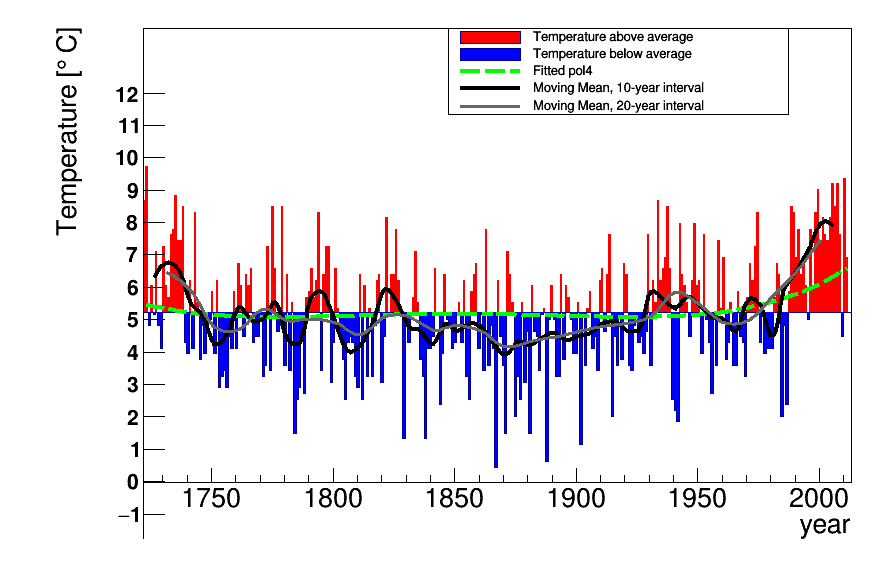
\includegraphics[scale=0.4]{tempYear.png}
    \caption{Histogram showing the annual average temperatures in Uppsala and surroundings from $1722$ to $2013$. The average temperature over the whole period is $5.2$ celsius. Temperatures above this total average are shown in red, those below are shown in blue. Two moving averages ("Moving Mean") are shown as solid black and gray lines, and a fit of a polynomial of fourth degree is shown as a green dashed line.}
   \label{fig:year}
\end{figure}
If you use the function tempPerplotandpred(2050) it gives you an extrapolated value of 7.5 degrees Celsius.
The reduced $\chi^2 \approx 0.8$ for the polynomial fit, suggesting a slight underfitting, which is hardly surprising as the annual temperature average has chaotic fluctuations and is hard to fit with a linear continuous function.

\subsection{Part B:}

\subsection{Part C: Which is the hottest and coldest day most likely to occur in one of the locations in Uppsala?}

\item The warmest and coldest day of each year
\begin{figure}[H]
    \centering
    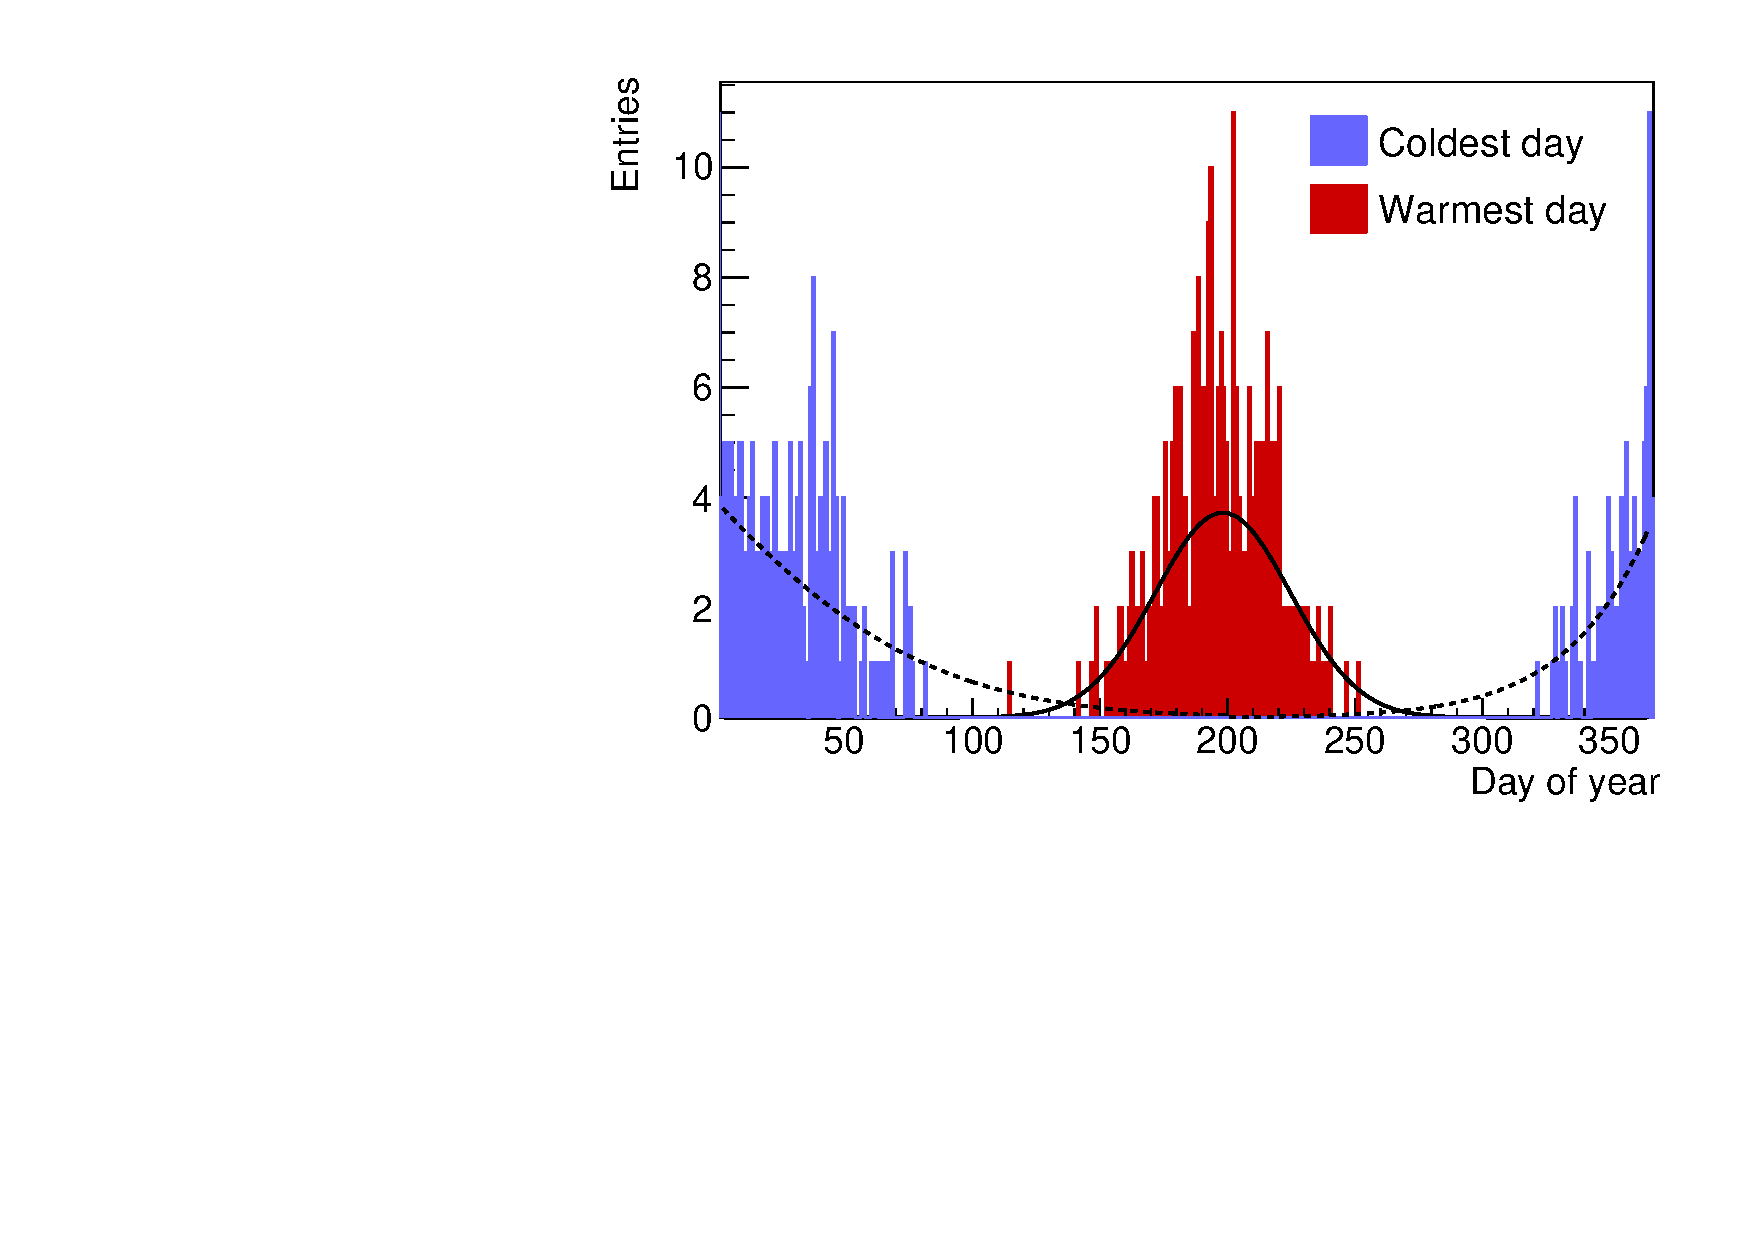
\includegraphics[width=8cm]{./images/hotCold_Upp_final}
    \caption{final histogram}
    \label{fig:hist}
\end{figure}
As the histogram shows, the most likely coldest day is on the end of the year (31/12), and the most likely hottest day is on 13/7.

\section{Discussion}\label{sec:discussion}
\subsection{Part A: The rising temperature in Uppsala and surroundings}
From Fig. \ref{fig:year} it is clear that the average temperature is rising not only globally, but also on a local level in mid-Sweden. In this report we have confirmed concerns of global temperature rising using measurements from Uppsala and surroundings, but it would be interesting to compare with data from other places around the world, to see how the changes correlate. It would also be interesting to see which locations are more affected by the global warming than others. This is left for future research.

\subsection{Part B:}
From Figure X we can see that the number of days bellow 0 C each year varies quite a bit, but there seams to be a trend down, which would make sense as when the earth gets hotter do to global warming the number of days bellow 0 C would naturally decrees. There seams to be a periodicity in the fluctuations, but the data is to noisy for a sin fit so we did not do one.  To say it with confidence is not possible as the number of years and the variance in the values makes it.

\subsection{Part C: The warmest and coldest day of each year}

The question is to try to find out the possibilities of dates to become the hottest and coldest date. We read the data of Uppsala and then plot the histogram of the occurrence for each date being hottest or coldest. 

\begin{figure}[htp]
    \centering
    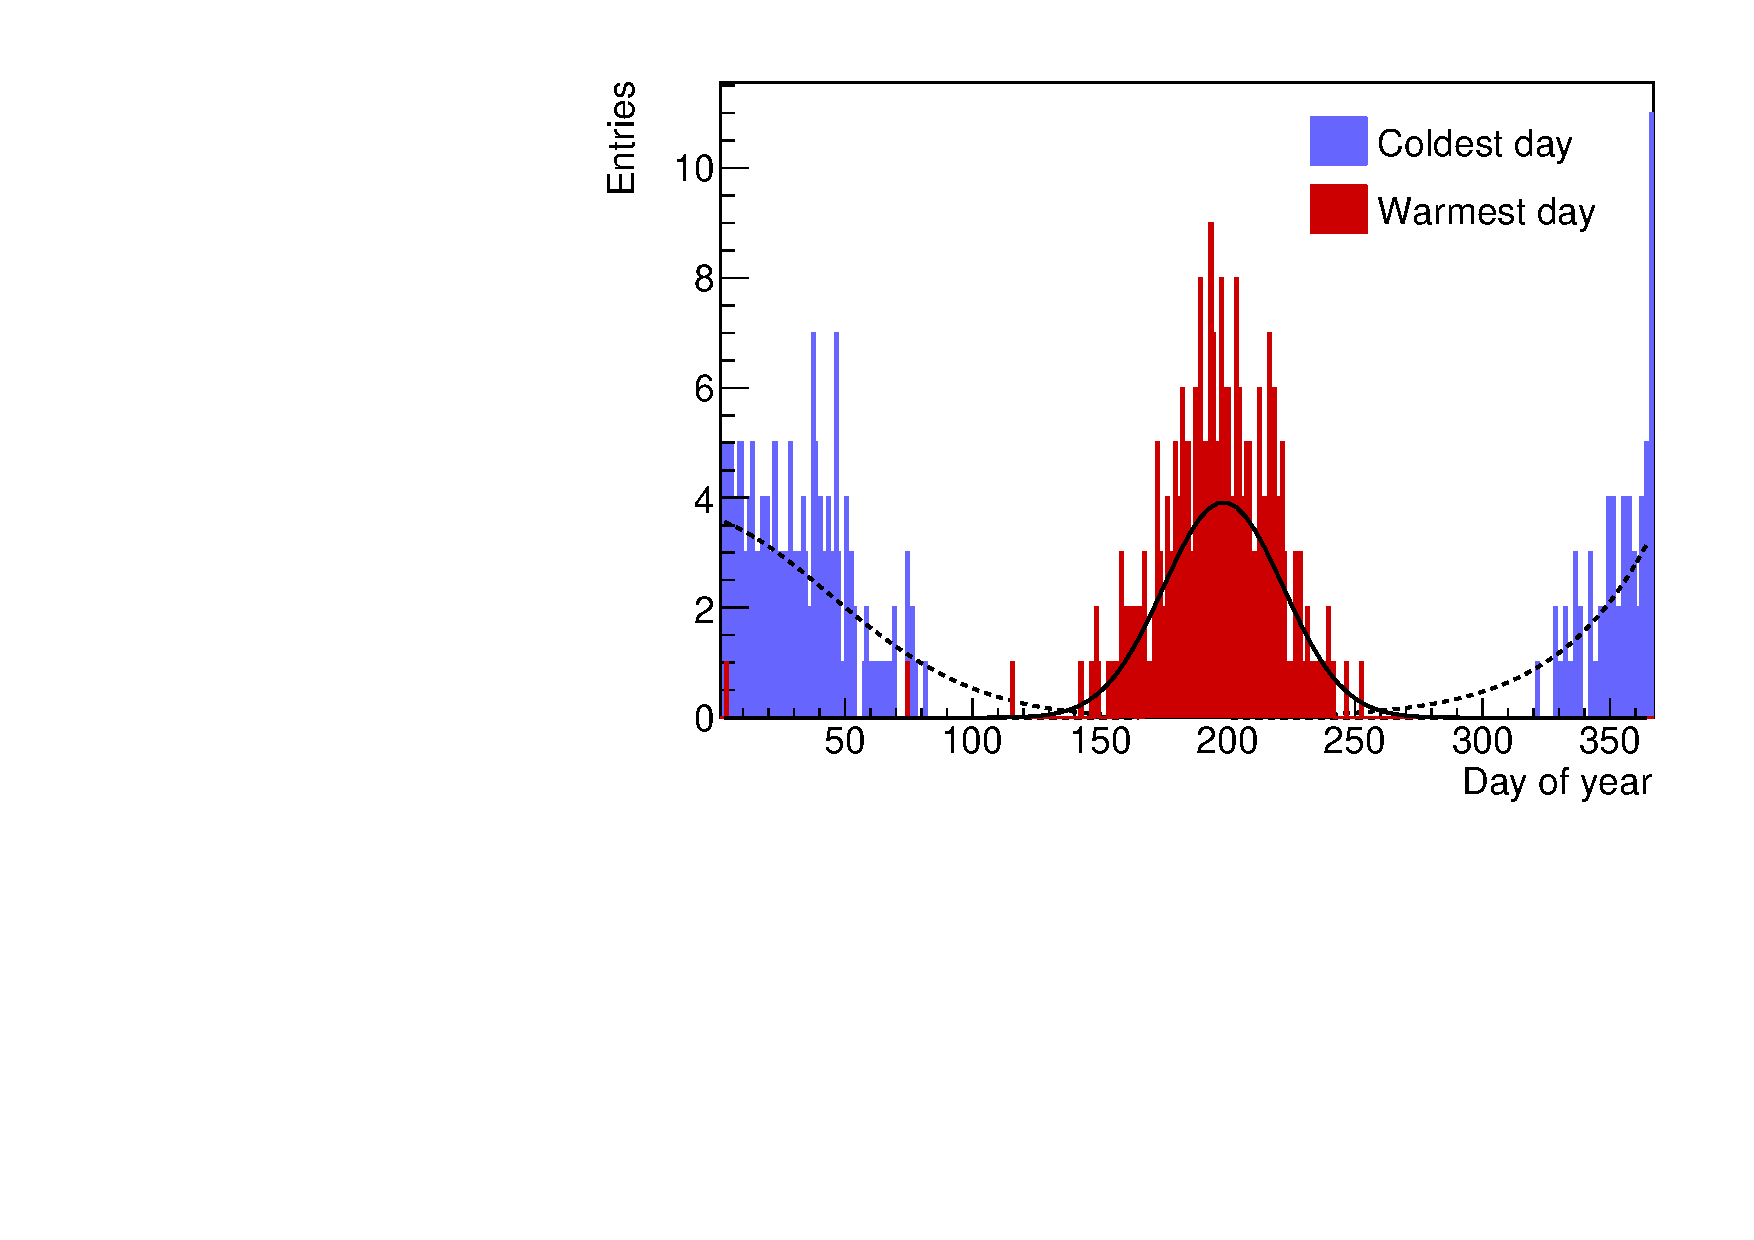
\includegraphics[width=8cm]{./images/hotCold_Upp_prev}
    \caption{first histogram}
    \label{fig:hist}
\end{figure}

We noticed some problem:
\begin{enumerate}
\item There are some coldest date in summer, and also some hottest date in winter, which isn't make sense.
\item Winter is distributed at the first and the end of the year, so we use two Gaussian function to fit on those two parts. However, the plot should be circular in practice. We should take both parts into consideration when we draw fit line.
\end{enumerate}
Then we figured out the cause of the first problem. Because the Uppsala data set is a combination of some places around Uppsala. For this question, we ignored those places other than Uppsala. This makes the data became uncomplete. For example, data of 1766 are all from Stockholm after April 5, thus the hottest date in 1766 would be April 4, which does not make sense. To solve this, we only accept coldest days which is less than 100 or more than 300 in day of the year, and hottest days which is between 100 and 300 in day of the year.




The graph from the problem where we calculated the number of days that had average temperature bellow 0 clearly shows some anomaly in the first few point. It has to do with bad data. The cvs file denoted the quality of the with G for good and bad with Y 



To solve the second problem, we extend the length of the x-axis of histogram to 732, twice of a year. Then we just copy the tail to the front, and also the front to the tail. We plot two Gaussian fit lines for coldest date, one at the front and the other one at the end, and these line must be the same. By doing so, we can take all the coldest date into consideration. Finally, we just need to combine all the fit lines in same plot, and only take from day 1 to day 366 and ignore others.
\begin{figure}[htp]
    \centering
    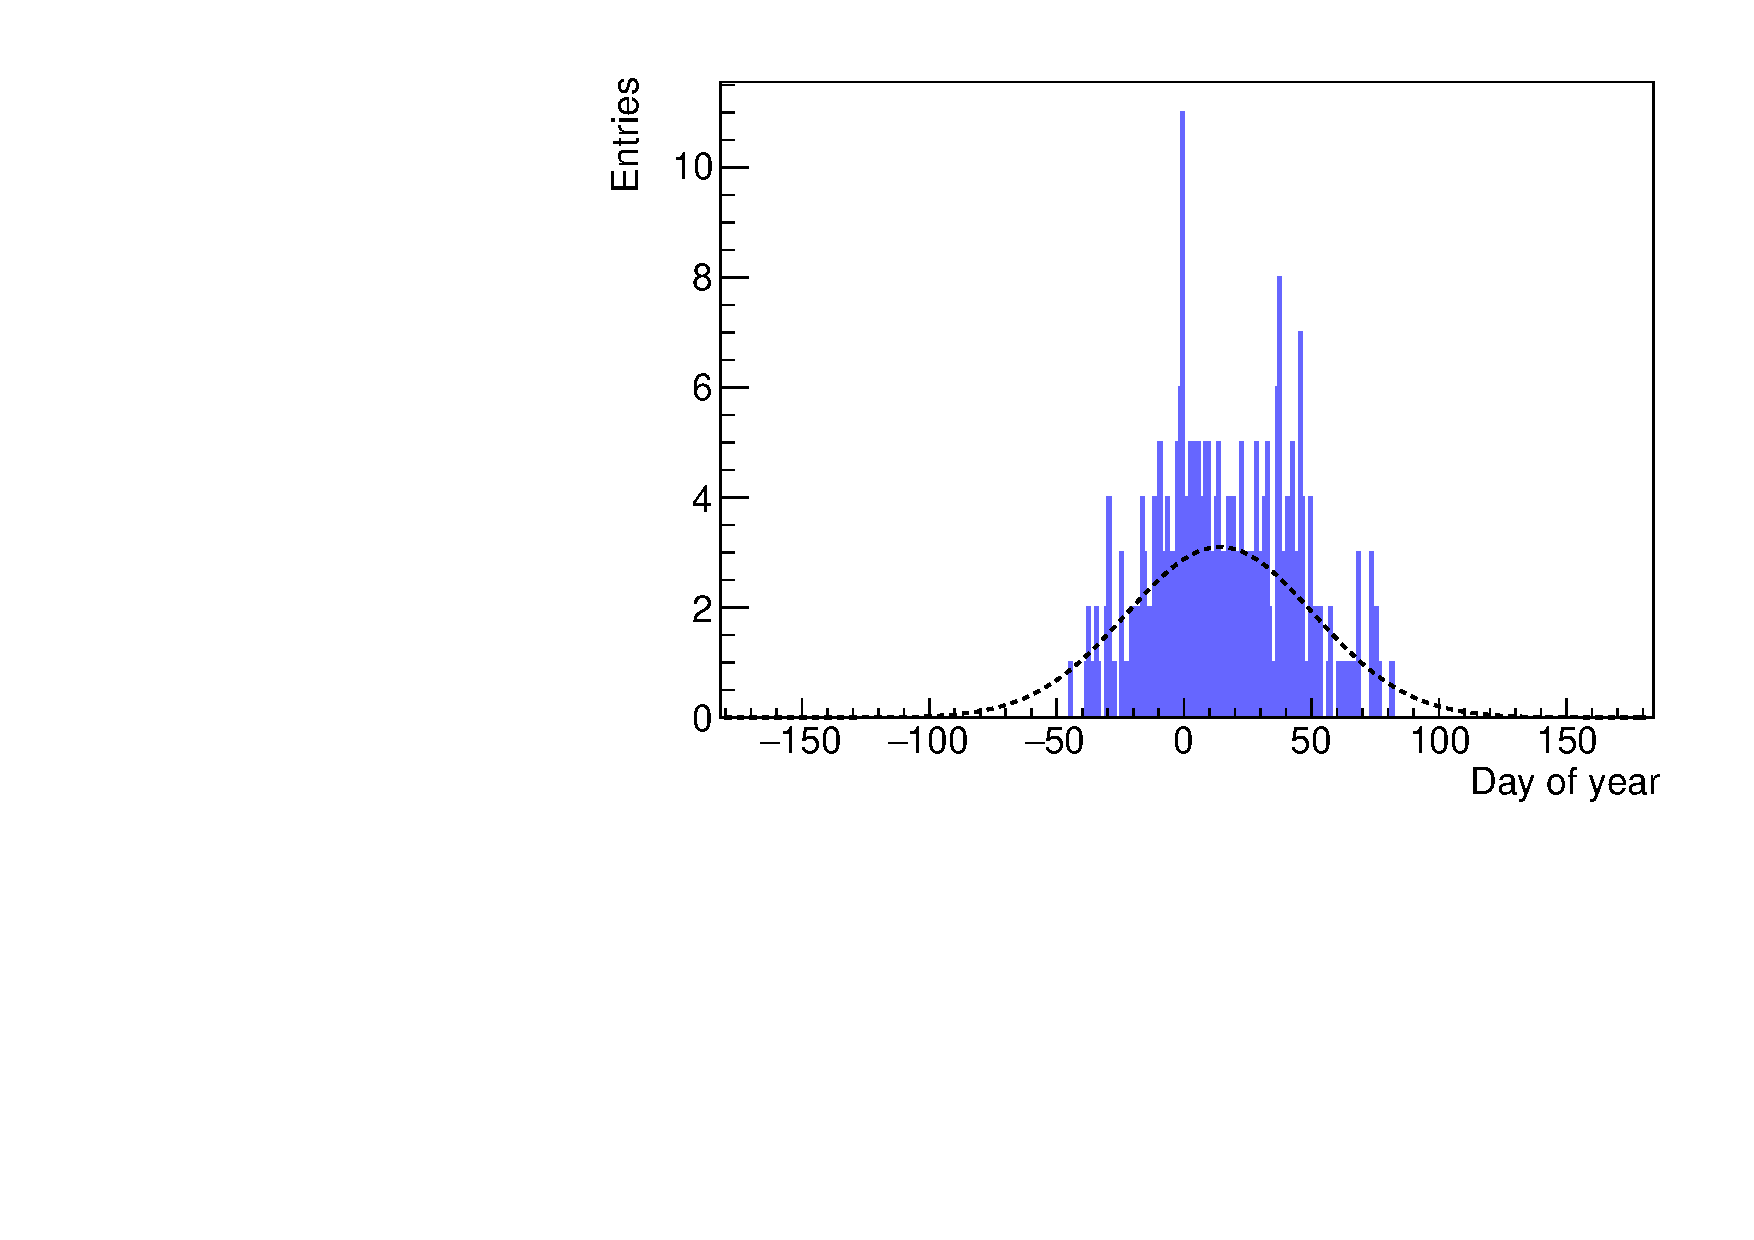
\includegraphics[width=8cm]{./images/hotCold_Upp_cold_1}
    \caption{extended histogram at the begin of the year}
    \label{fig:hist}
\end{figure}
\begin{figure}[htp]
    \centering
    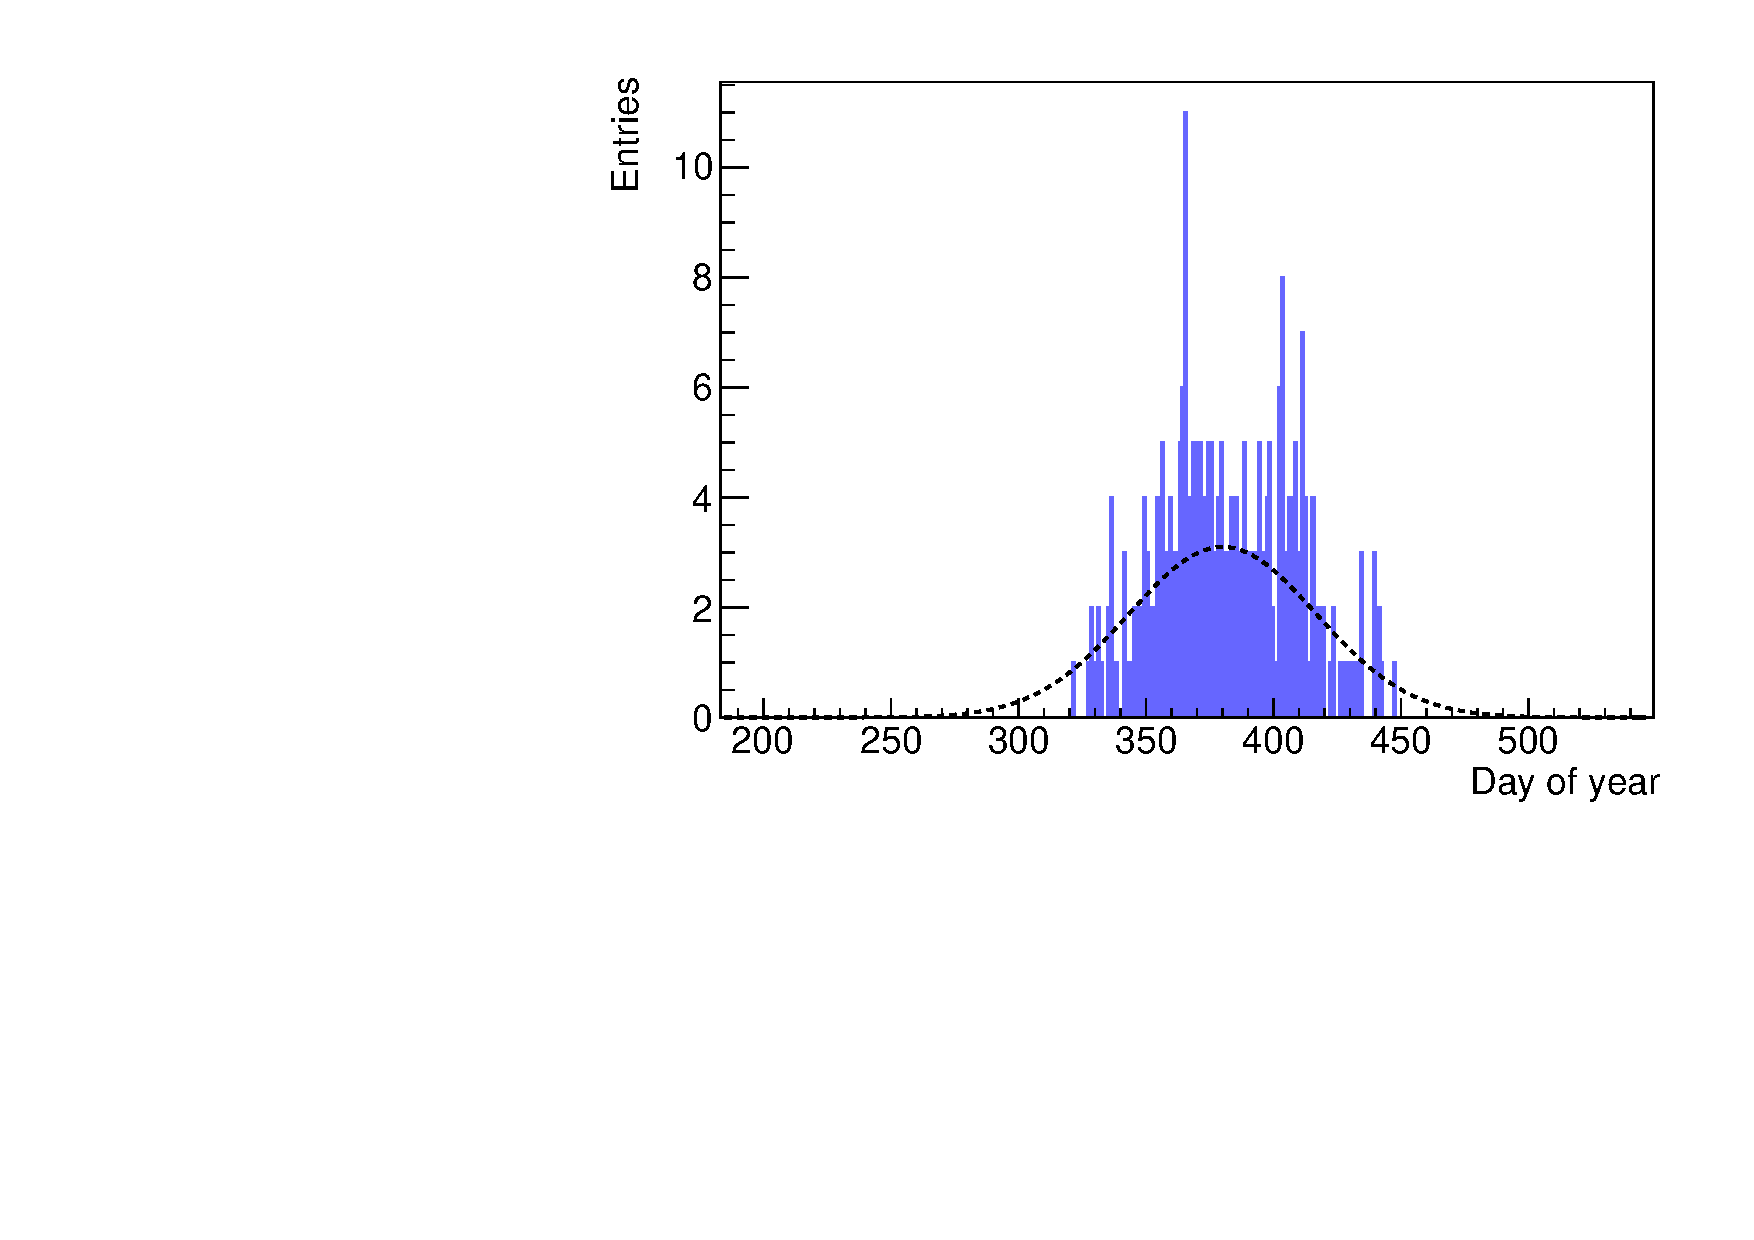
\includegraphics[width=8cm]{./images/hotCold_Upp_cold_2}
    \caption{extended histogram at the end of the year}
    \label{fig:hist}
\end{figure}
\begin{figure}[htp]
    \centering
    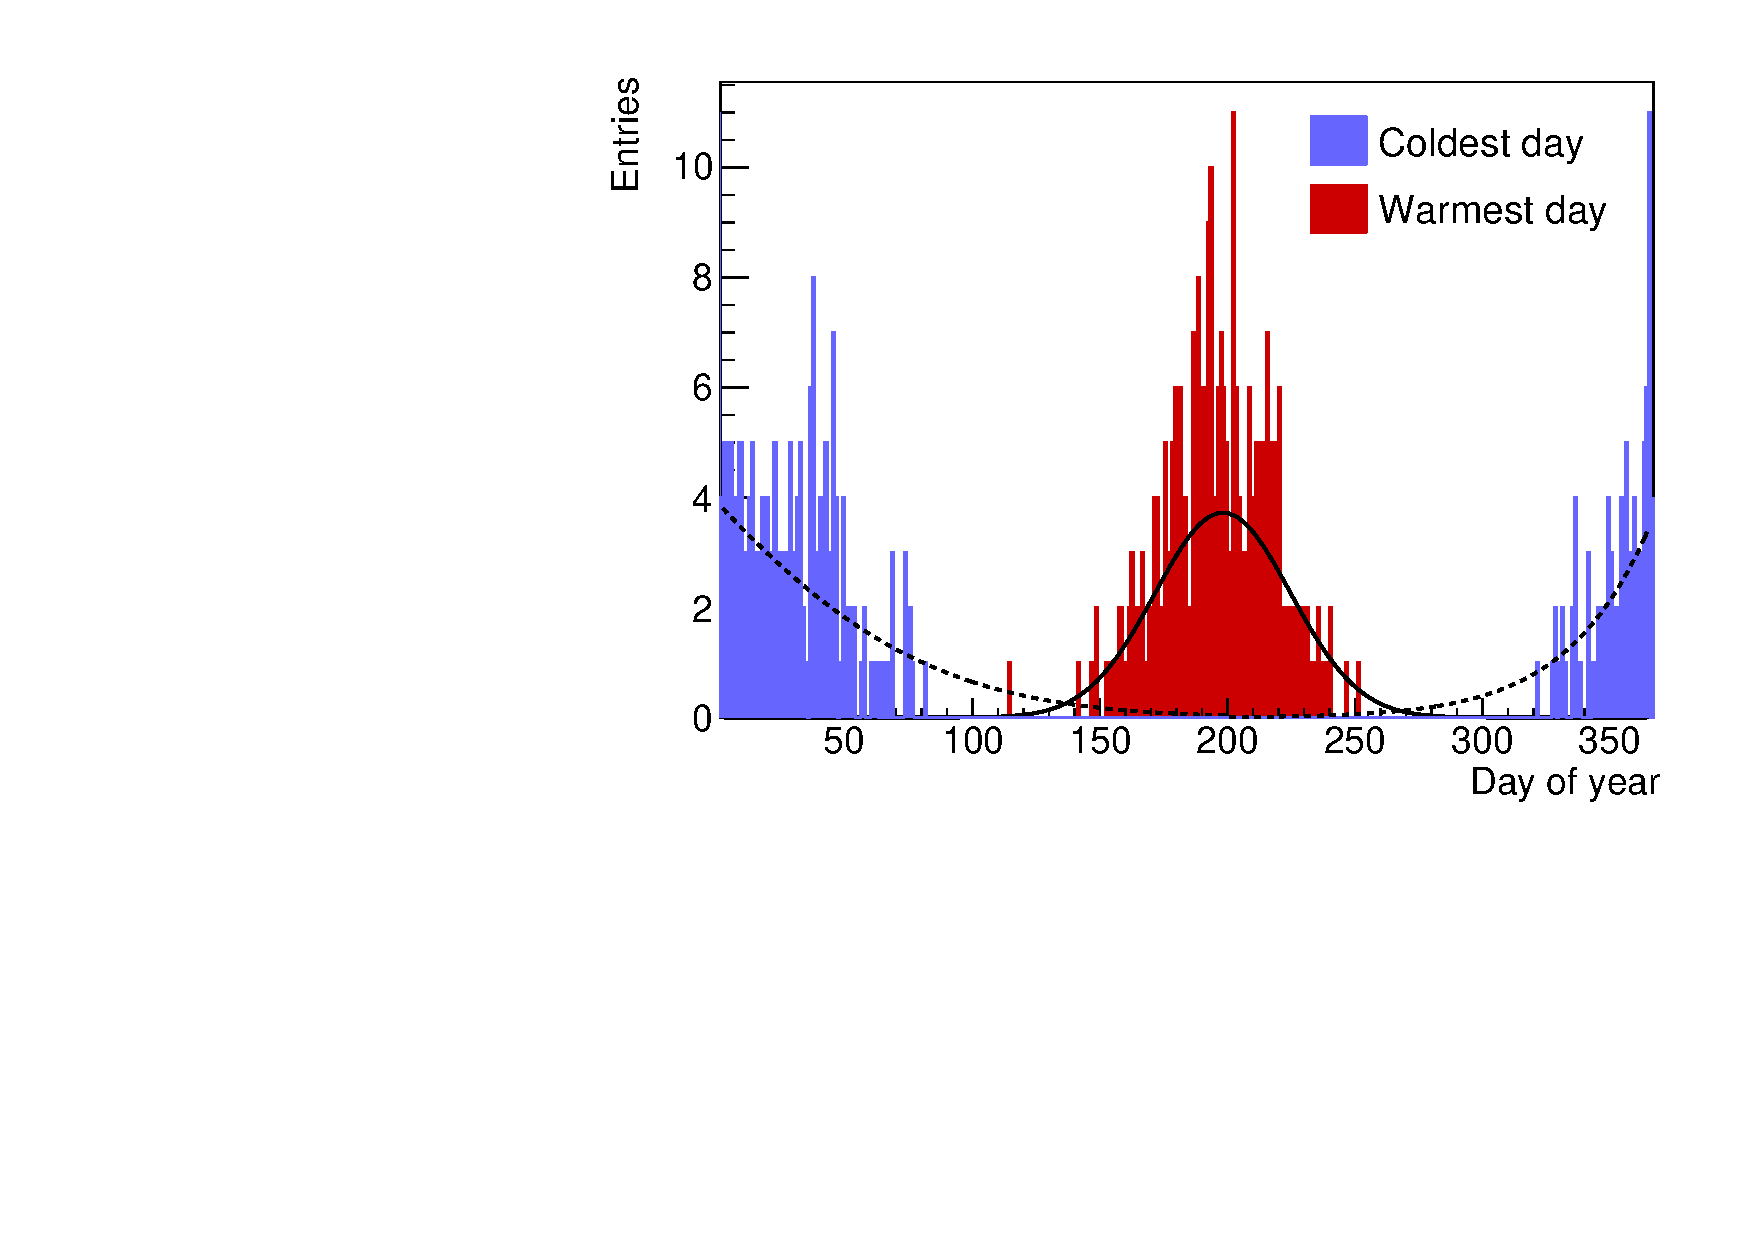
\includegraphics[width=8cm]{./images/hotCold_Upp_final}
    \caption{final histogram}
    \label{fig:hist}
\end{figure}




\end{document}

    © 2019 GitHub, Inc.
    Terms
    Privacy
    Security
    Status
    Help

    Contact GitHub
    Pricing
    API
    Training
    Blog
    About

